\documentclass[border=10px]{standalone}
\usepackage{tikz}
\usetikzlibrary{patterns}
\usetikzlibrary{shapes.arrows}
\usepackage{amssymb}
\usetikzlibrary{calc}
\usepackage{verbatim}
\usetikzlibrary{positioning}
\tikzset{sign/.style={black, inner sep = 0pt, minimum width = 0mm, text width = 5mm, fill=green!20, font=\bfseries,  minimum height = 8mm,  align = center}}
\usepackage{lcd}
\begin{document}
	
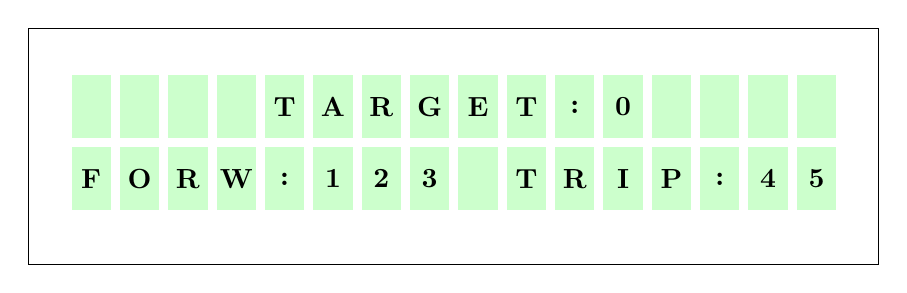
\begin{tikzpicture}[scale=1]
  \draw[draw = black] (-0.8,1) rectangle (10,-2); 
  \node[sign] (n0) {};
  \foreach \x/\t [remember=\x as \lastx (initially 0)] in {1/ , 2/ , 3/ , 4/T , 5/A , 6/R , 7/G , 8/E , 9/T , 10/: , 11/0 , 12/ , 13/ , 14/ , 15/}{
    \node[sign, right = 1mm of n\lastx] (n\x) {\t};
  }

  \node[sign, below = 1mm of n0] (m0) {F};
  \foreach \x/\t [remember=\x as \lastx (initially 0)] in {1/O, 2/R, 3/W, 4/:, 5/1, 6/2 , 7/3, 8/ , 9/T, 10/R, 11/I, 12/P, 13/:, 14/4, 15/5}{
  \node[sign, right = 1mm of m\lastx] (m\x) {\t};
}


\end{tikzpicture}
	
\end{document}
